\documentclass[dvipdfmx]{jlreq}

\usepackage[dvipdfmx]{graphicx}
\usepackage[hidelinks]{hyperref}
\usepackage{float}
\usepackage{svg}
\usepackage{booktabs}
\usepackage{longtable}
\usepackage{array}

\begin{document}

\input{sections/title}
\newpage

\tableofcontents
\clearpage

% はじめに

% システム概要

% コーディング規約

% 動作環境

% 開発環境
\section{動作環境}
\subsection{ソフトウェア環境}
本システムにおけるソフトウェアの構成を表\ref{tab:SoftwareConfig}に示す.

\begin{table}
    \centering
    \caption{ソフトウェア構成}
    \label{tab:SoftwareConfig}
    \begin{tabular}{l|l}
        \hline
        項目 & ソフトウェア \\
        \hline
        \hline
        メインサーバ & Ubuntu \\
        データサーバ & Amazon Aurora\\
        APサーバ & Nginx \\
        Webサーバ & Nginx \\
        バックエンド & Go \\
        フロントエンド & React \\
        事業者端末 & Windows \\
        利用者端末 & Google Chrome, Safari, Microsoft Edge 等の主要ブラウザ \\ 
        \hline
    \end{tabular}
\end{table}
\section{開発環境}
本システムの開発環境を表\ref{}に示す.

\begin{table}
    \centering
    \caption{開発環境}
    \label{fig:DevelopmentEnvironment}
    \begin{tabular}{|l|l|l|}
        \hline
        項目 & 詳細 & 備考 \\
        OS & Windows 11 Home & 開発端末 \\
        エディター & VisualStudioCode & システム開発に使用 \\
        バージョン管理 & GitHub & ソースコード管理 \\
        プログラミング言語 & HTML, CSS, TypeScript, Go & Webアプリケーション開発 \\
        データベース & MySQL & データ保存および操作 \\
        \hline

% モジュール設計
\section{モジュール設計}

% モジュール一覧
\subsection{モジュール一覧}
本システムのモジュール一覧を表\ref{tab:commonmodule}から\ref{tab:adminmodule}に示す.モジュールIDはM(共通:1,利用者:2,事業者:3,管理者:4)-(各機能の番号)-(もし,同じ機能で分けられているモジュールがあるならば,仕様順番の番号)となっている.

\begin{longtable}{|c|c|>{\hspace{0pt}\centering\arraybackslash}p{5cm}|}
    \caption{共通モジュール一覧}
    \label{tab:commonmodule} \\ 

    \hline
    \endhead
    
    \hline
    \endfoot
    
    \hline
    \endlastfoot
    
    \hline
        モジュールID & モジュール名 & 概要 \\ \hline
        M1-1 & LoginScreen & ログイン画面を表示する \\ \hline
        M1-2 & FetchMemberInfo & 会員情報を取得する \\ \hline
        M1-3-1 & SelectLogout & ログアウトを選択 \\ \hline
        M1-3-2 & LogoutScreen & ログアウト画面を表示 \\ \hline
        M1-3-3 & Logout & ログアウトする \\ \hline
        M1-4-1 & SelectWithdrawal & 退会を選択 \\ \hline
        M1-4-2 & WithdrawalScreen & 退会画面を表示 \\ \hline
        M1-4-3 & Withdrawal & 退会処理をする \\ \hline
        M1-5-1 & ContactScreen & お問い合わせ画面を表示 \\ \hline
        M1-5-2 & InputContactForm & お問い合わせ内容を入力 \\ \hline
        M1-5-3 & SubmitContact & お問い合わせ内容を格納 \\ \hline
        M1-6-1 & GetPostList & 投稿一覧を取得 \\ \hline
        M1-6-2 & CheckPostCountThreshold & 投稿数が50以上か判定 \\ \hline
        M1-6-3 & MapViewScreen & 地図表示画面を表示 \\ \hline
        M1-7-1 & SelectPin & ピンを選択 \\ \hline
        M1-7-2 & GetPostDetail & 投稿内容を取得 \\ \hline
        M1-7-3 & DisplayPostList & 投稿閲覧画面を表示 \\ \hline
        M1-8-1 & GetLocation & 位置情報を取得 \\ \hline
        M1-8-2 & NewPostScreen & 新規投稿画面を表示 \\ \hline
        M1-8-3 & GetPostTimestamp & 投稿した日時を取得 \\ \hline
        M1-8-4 & SubmitPostDetail & 投稿内容を格納 \\ \hline
        M1-9-1 & SelectBlock & ブロックを選択 \\ \hline
        M1-9-2 & SubmitBlock & ブロック情報を格納 \\ \hline
        M1-10-1 & SelectUnlock & ブロック解除を選択 \\ \hline
        M1-10-2 & DeleteBlock & ブロック情報を削除 \\ \hline
        M1-11-1 & GetBlockList & ブロックリストを取得 \\ \hline
        M1-11-2 & UserBlockViewScreen & ブロックリストを表示 \\ \hline
        M1-12-1 & ReportScreen & 通報画面を表示 \\ \hline
        M1-12-2 & SubmitReport & 通報内容を格納 \\ \hline
        M1-13-1 & SelectPostDeletion & 自分の投稿の削除を選択 \\ \hline
        M1-13-2 & DeletePostDetail & 投稿内容を削除 \\ \hline
        M1-14-1 & SelectPostHistory & 投稿履歴を選択 \\ \hline
        M1-14-2 & GetPostHistory & 投稿履歴を取得 \\ \hline
        M1-14-3 & DisplayPostHistory & 投稿履歴を表示 \\ \hline
        M1-15-1 & SelectUserSetting & 設定を選択 \\ \hline
        M1-15-2 & DisplayUserSetting & 設定を表示 \\ \hline
\end{longtable}

\begin{longtable}{|c|c|>{\hspace{0pt}\centering\arraybackslash}p{5cm}|}
    \caption{一般会員モジュール一覧}
    \label{tab:usermodule} \\
    \hline
    モジュールID & モジュール名 & 概要 \\ \hline
    M2-1 & UserInputInformation & Google認証にアクセスして,DBに利用者情報を格納または,ログインをする \\ \hline
    M2-2-1 & UserSelectMyPage & マイページを選択 \\ \hline
    M2-2-2 & UserDisplayMyPage & マイページ画面を表示 \\ \hline
    M2-3-1 & UserInputSearchKeyword & キーワードを入力する \\ \hline
    M2-3-2 & KeywordSearch & キーワード検索をする \\ \hline
    M2-3-3 & UserDisplayKeywordSearchResults & キーワード検索結果を表示 \\ \hline
    M2-4-1 & UserSelectSearchGenre & ジャンルを選択 \\ \hline
    M2-4-2 & GenreSearch & ジャンル検索をする \\ \hline
    M2-4-3 & UserDisplayGenreSearchResults & ジャンル検索結果を表示 \\ \hline
    M2-5-1 & UserSelectSearchPeriod & 期間を選択 \\ \hline
    M2-5-2 & DateSearch & 期間検索をする \\ \hline
    M2-5-3 & UserDisplayPeriodSearchResults & 期間検索結果を表示\\ \hline
    M2-6-1 & UserTriggerReaction & リアクションボタンを押す \\ \hline
    M2-6-2 & UserInputReactionInformation & リアクション情報を格納 \\ \hline
    M2-7-1 & UserInputBusinessApplication & 事業者申請を入力 \\ \hline
    M2-7-2 & InputBusinessRequestInformation & 事業者申請を格納 \\ \hline
    M2-8-1 & UserGetReactionList & リアクション履歴を取得 \\ \hline
    M2-8-2 & UserReactionViewScreen & リアクション履歴を表示 \\ \hline
\end{longtable}

\begin{longtable}{|c|c|>{\hspace{0pt}\centering\arraybackslash}p{5cm}|}
    \caption{事業者会員モジュール一覧}
    \label{tab:busmodule} \\
    \hline
    モジュールID & モジュール名 & 概要 \\ \hline
    M3-1 & BusinessInputInformation & Google認証にアクセスして \par ログインする \\ \hline
    M3-2-1 & BusinessSelectMyPage & マイページ画面を選択 \\ \hline
    M3-2-2 & BusinessGetMyPageDetails & 事業者会員情報の取得 \par (マイページ画面用) \\ \hline
    M3-2-3 & BusinessDisplayMyPage & マイページ画面を表示する \\ \hline
    M3-3 & BusinessDeleteInformation & 会員情報を削除する \\ \hline
    M3-4-1 & InputNewBusinessName & 変更する事業者名を入力する \\ \hline
    M3-4-2 & UpdateBusinessName & 変更した事業者名を格納する \\ \hline
    M3-4-3 & ChangeBusinessNameScreen & 事業者名の変更を反映する \\ \hline
    M3-5-1 & InputNewBusinessIcon & 変更する事業者アイコンを入力する \\ \hline
    M3-5-2 & UpdateBusinessIcon & 変更した事業者アイコンを格納する \\ \hline
    M3-5-3 & ChangeBusinessIconScreen & 事業者アイコンの変更を反映する \\ \hline
    M3-6 & BusinessRedirectToStripe & Stripeにリダイレクトする \\ \hline
    M3-7-1 & BusinessGetTotalPostNumber & 総投稿数を取得する \\ \hline
    M3-7-2 & BusinessGetTotalReactionNumber & 総リアクション数を取得する \\ \hline
    M3-7-3 & BusinessGetTotalViewNumber & 総閲覧数を取得する \\ \hline
    M3-7-4 & BusinessGetEngagement & エンゲージメント率を計算する \\ \hline
    M3-7-5 & BusinessDashboardScreen & ダッシュボード画面を表示する \\ \hline
    M3-7-6 & BusinessDashboardGraphScreen & 週間推移をグラフで表示する \\ \hline
    M3-7-7 & BusinessDisplayTopReactions & リアクション数が多い投稿5つを表示する \\ \hline
\end{longtable}

\begin{longtable}{|c|c|>{\hspace{0pt}\centering\arraybackslash}p{5cm}|}
    \caption{管理者モジュール一覧}
    \label{tab:adminmodule} \\
    \hline
    モジュールID & モジュール名 & 概要 \\ \hline
    M4-1 & AdminInputInformation & Google認証にアクセスして \par ログインする \\ \hline
    M4-2-1 & AdminSelectLogout & ログアウトを選択 \\ \hline
    M4-2-2 & AdminLogout & ログアウトする \\ \hline
    M4-3-1 & AdminGetTotalUserNumber & 総ユーザー数を取得する \\ \hline
    M4-3-2 & AdminGetActiveUserNumber & アクティブユーザー数を取得する \\ \hline
    M4-3-3 & AdminGetTotalPostNumber & 総投稿数を取得する \\ \hline
    M4-3-4 & AdminGetTotalReactionNumber & 総リアクション数を取得する \\ \hline
    M4-3-5 & AdminGetBusinessAccountNumber & 事業者アカウント数を取得する \\ \hline
    M4-3-6 & AdminGetNotReportNumber & 未処理通報数を取得する \\ \hline
    M4-3-7 & AdminDashboardScreen & 概要画面を表示する \\ \hline
    M4-3-8 & AdminDashboardGraphScreen & 週間アクティビティ推移と \par ジャンル別投稿をグラフで表示する \\ \hline
    M4-4-1 & AdminGetReportDetails & 通報情報を取得する \\ \hline
    M4-4-2 & AdminDisplayReportManagement & 通報管理画面を表示する \\ \hline
    M4-4-3 & ProcessReportScreen & 通報を「処理済み」にする \\ \hline
    M4-5-1 & AdminGetBusinessApplications & 事業者申請情報を取得する \\ \hline
    M4-5-2 & AdminDisplayBusinessApplicationList & 事業者申請画面を表示する \\ \hline
    M4-5-3 & AdminDeleteApplicationData & 申請情報を削除する \\ \hline
    M4-5-4 & ProcessBusinessRequestScreen & 対応した事業者申請を \par 反映させる \\ \hline
    M4-6-1 & AdminGetUserDetails & ユーザー情報を取得する \\ \hline
    M4-6-2 & AdminDisplayUserManagement & ユーザー管理画面を表示する \\ \hline
    M4-6-3 & AdminSelectUserDeletion & ユーザー一覧から削除ボタンを選択する \\ \hline
    M4-6-4 & AdminDeleteAccount & アカウントを削除する \\ \hline
    M4-6-5 & SendUserMessage & 利用者に通知を送信する \\ \hline
    M4-6-6 & AdminUpdateUserListUI & ユーザー一覧に処理を反映する \\ \hline
    M4-7-1 & AdminGetContactMessages & お問い合わせ情報を取得する \\ \hline
    M4-7-2 & AdminDisplayContactManagement & お問い合わせ画面を表示する \\ \hline
    M4-7-3 & ProcessContact & 問い合わせに対応して \par 「対応済み」にする \\ \hline
    M4-7-4 & ProcessContactScreen & 対応した問い合わせを反映する \\ \hline
\end{longtable}

% 一般会員側モジュール
\subsection{一般会員側モジュール}


% 事業者側モジュール
\subsection{事業者側モジュール}
\subsubsection{GetPayInformation}
\begin{figure}[H]
    \centering
    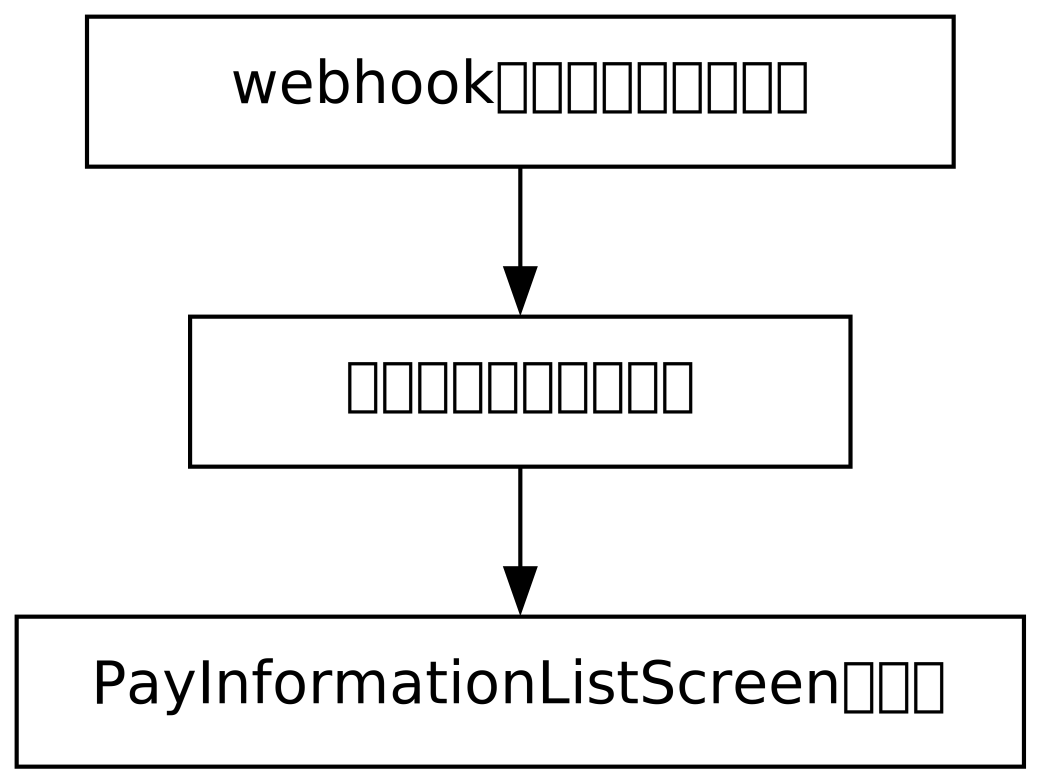
\includegraphics[keepaspectratio, width=0.8\linewidth]{figures/sato/GetPayInformation.pdf}
    \caption{GetPayInformation}
    \label{fig:GetPayInformation}
\end{figure}
\subsubsection{BusinessGetTotalPostNumber}
\begin{figure}[H]
    \centering
    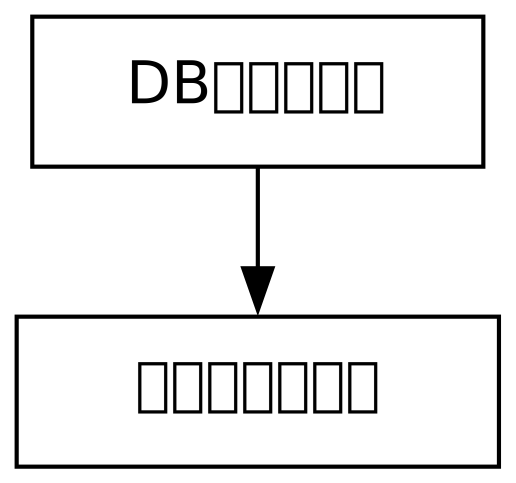
\includegraphics[keepaspectratio, width=0.8\linewidth]{figures/sato/BusinessGetTotalPostNumber.pdf}
    \caption{BusinessGetTotalPostNumber}
    \label{fig:BusinessGetTotalPostNumber}
\end{figure}
\subsubsection{BusinessGetTotalReactionNumber}
\begin{figure}[H]
    \centering
    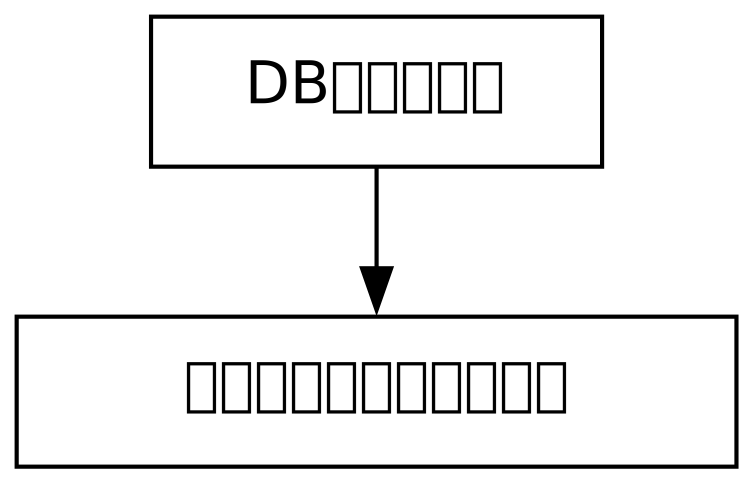
\includegraphics[keepaspectratio, width=0.8\linewidth]{figures/sato/BusinessGetTotalReactionNumber.pdf}
    \caption{BusinessGetTotalReactionNumber}
    \label{fig:BusinessGetTotalReactionNumber}
\end{figure}
\subsubsection{BusinessGetTotalViewNumber}

\begin{figure}[H]
    \centering
    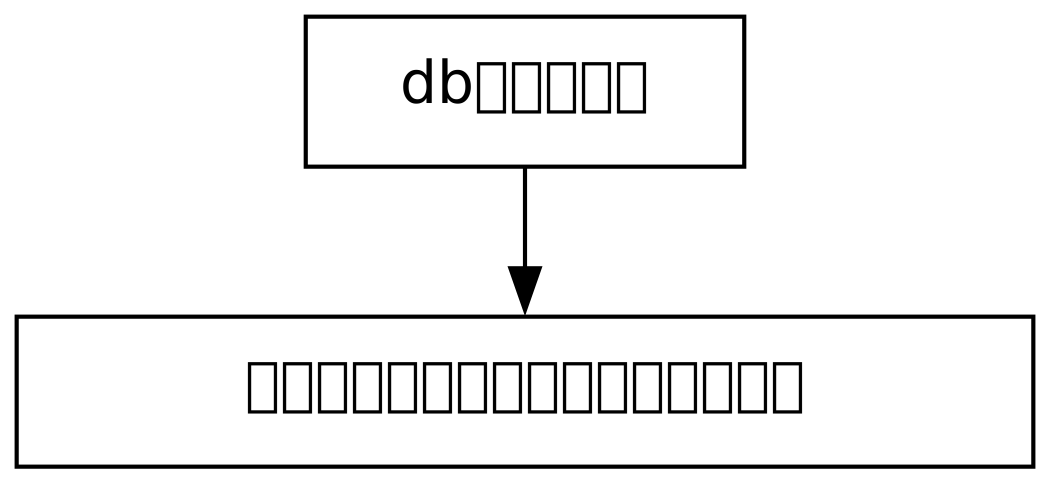
\includegraphics[keepaspectratio, width=0.8\linewidth]{figures/sato/BusinessGetTotalViewNumber.pdf}
    \caption{BusinessGetTotalViewNumber}
    \label{fig:BusinessGetTotalViewNumber}
\end{figure}
\subsubsection{BusinessGetEngagement}
\begin{figure}[H]
    \centering
    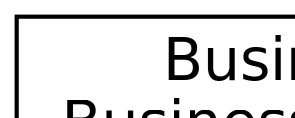
\includegraphics[keepaspectratio, width=0.8\linewidth]{figures/sato/BusinessGetEngagement.pdf}
    \caption{BusinessGetEngagement}
    \label{fig:BusinessGetEngagement}
\end{figure}

% 管理者側モジュール
\subsection{管理者側モジュール}
\subsubsection{AdminInputInformation}
\begin{figure}[H]
    \centering
    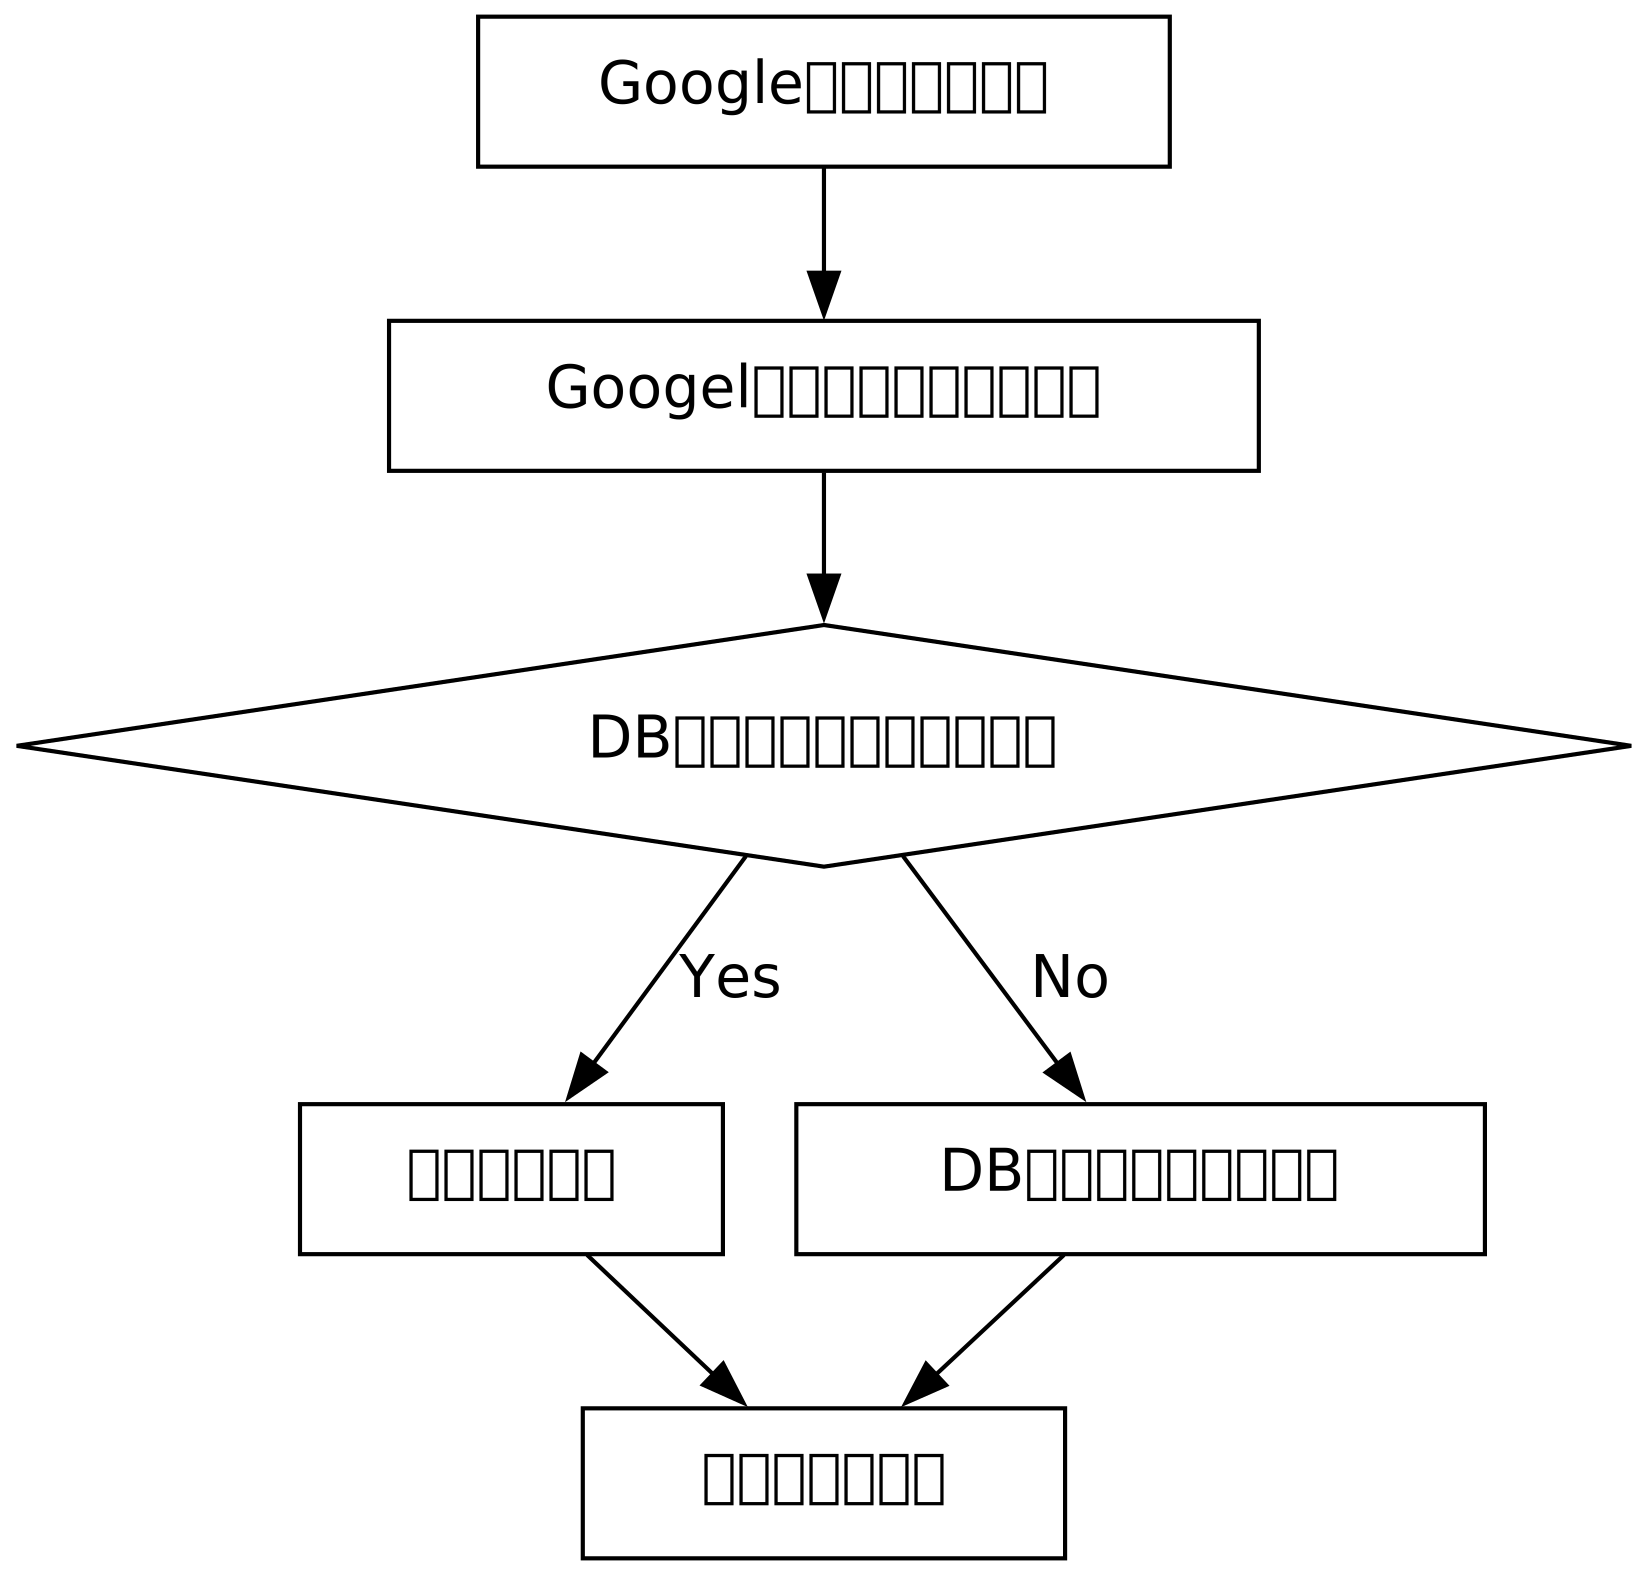
\includegraphics[keepaspectratio, width=0.8\linewidth]{figures/sato/AdminInputInformation.pdf}
    \caption{AdminInputInformation}
    \label{fig:AdminInputInformation}
\end{figure}
\subsubsection{AdminLogout}
\begin{figure}[H]
    \centering
    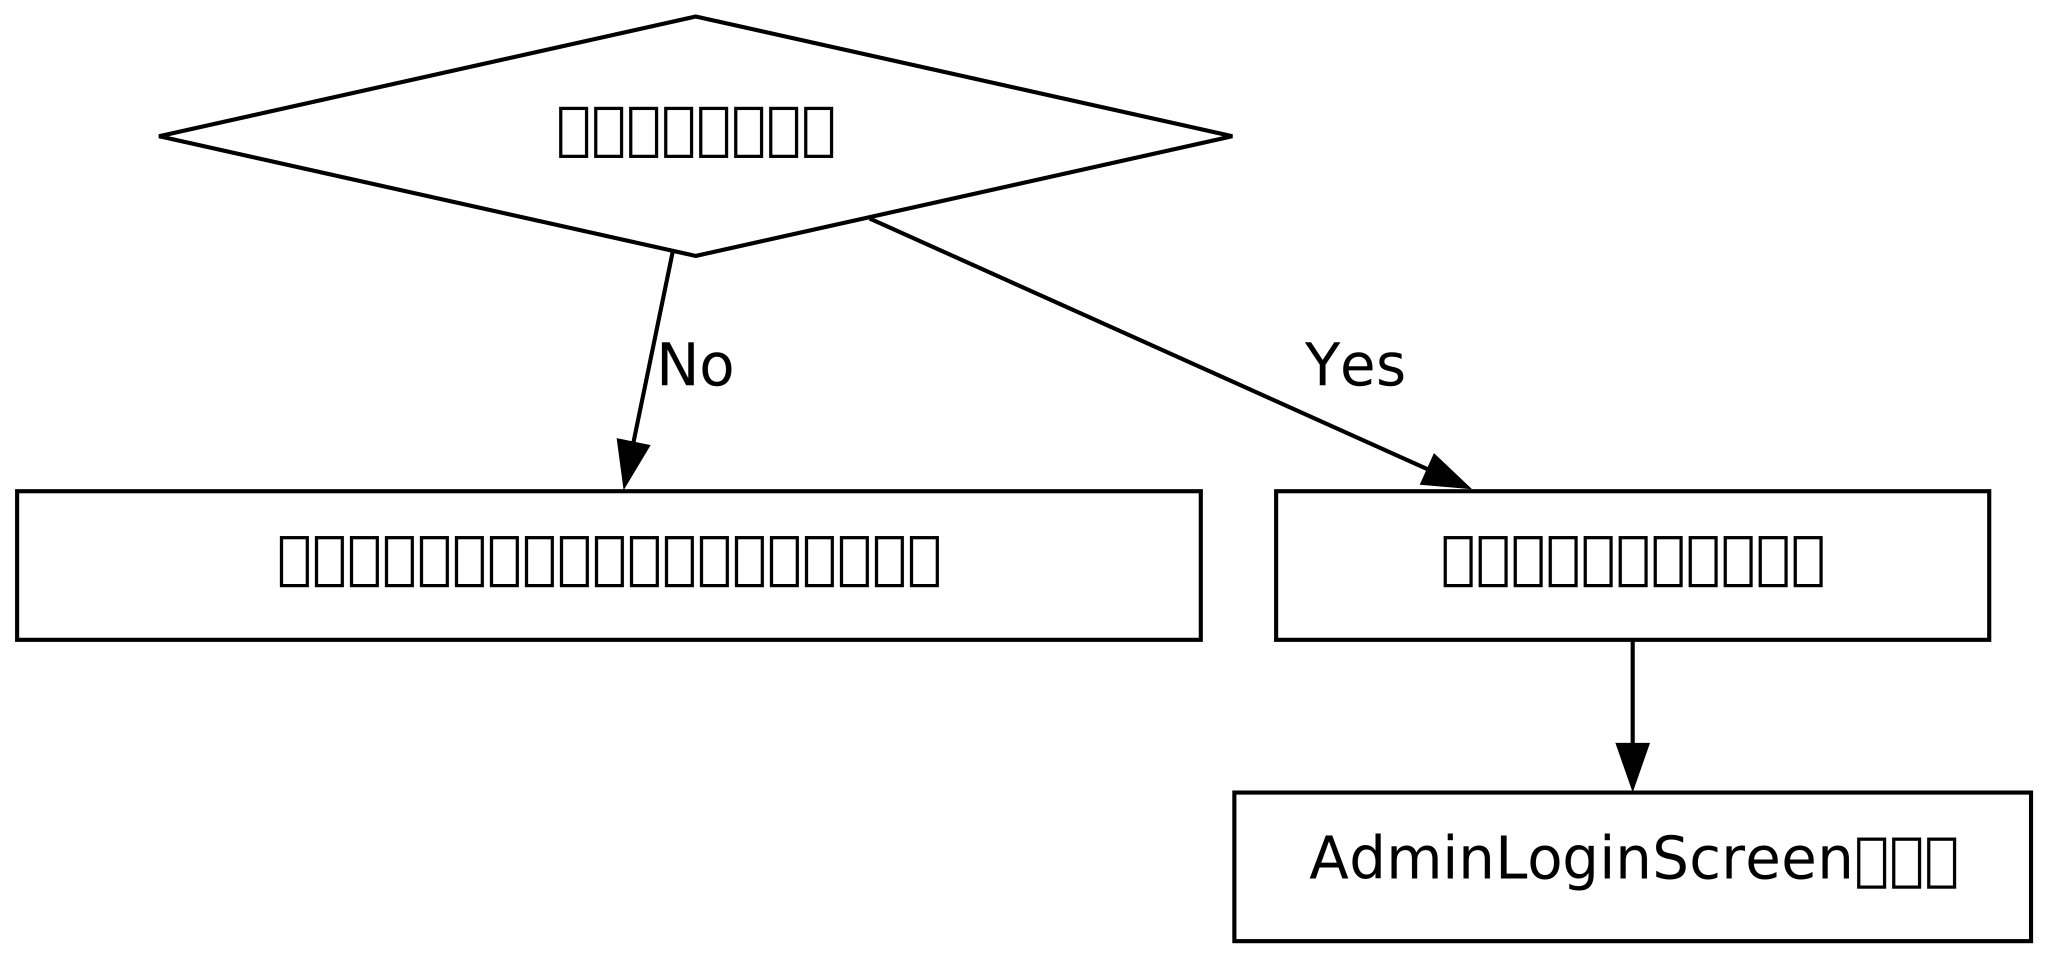
\includegraphics[keepaspectratio, width=0.8\linewidth]{figures/sato/AdminLogout.pdf}
    \caption{AdminLogout}
    \label{fig:AdminLogout}
\end{figure}
\subsubsection{AdminGetTotalUserNumber}
\begin{figure}[H]
    \centering
    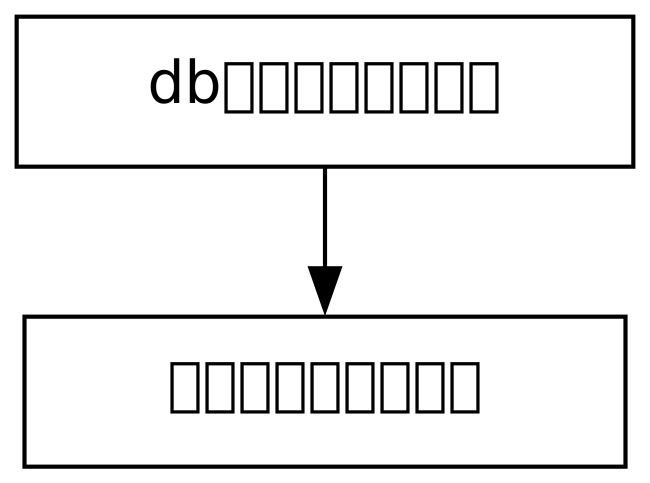
\includegraphics[keepaspectratio, width=0.8\linewidth]{figures/sato/AdminGetTotalUserNumber.pdf}
    \caption{AdminGetTotalUserNumber}
    \label{fig:AdminGetTotalUserNumber}
\end{figure}
\subsubsection{AdminGetActiveUserNumber}
\begin{figure}[H]
    \centering
    \includegraphics[keepaspectratio, width=0.8\linewidth]{figures/sato/AdminGetActiveUserNumber.pdf}
    \caption{AdminGetActiveUserNumber}
    \label{fig:AdminGetActiveUserNumber}
\end{figure}
\subsubsection{AdminGetTotalPostNumber}
\begin{figure}[H]
    \centering
    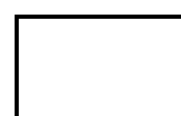
\includegraphics[keepaspectratio, width=0.8\linewidth]{figures/sato/AdminGetTotalPostNumber.pdf}
    \caption{AdminGetTotalPostNumber}
    \label{fig:AdminGetTotalPostNumber}
\end{figure}
\subsubsection{AdminGetTotalReactionNumber}
\begin{figure}[H]
    \centering
    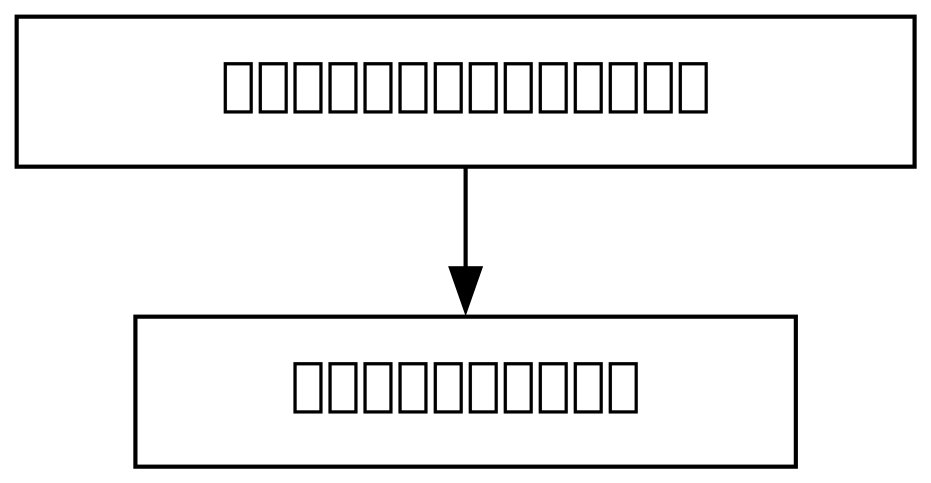
\includegraphics[keepaspectratio, width=0.8\linewidth]{figures/sato/AdminGetTotalReactionNumber.pdf}
    \caption{AdminGetTotalReactionNumber}
    \label{fig:AdminGetTotalReactionNumber}
\end{figure}
\subsubsection{AdminGetBusinessAccountNumber}
\begin{figure}[H]
    \centering
    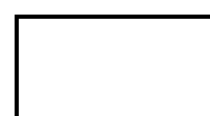
\includegraphics[keepaspectratio, width=0.8\linewidth]{figures/sato/AdminGetBusinessAccountNumber.pdf}
    \caption{AdminGetBusinessAccountNumber}
    \label{fig:AdminGetBusinessAccountNumber}
\end{figure}
\subsubsection{AdminGetNotReportNumber}
\begin{figure}[H]
    \centering
    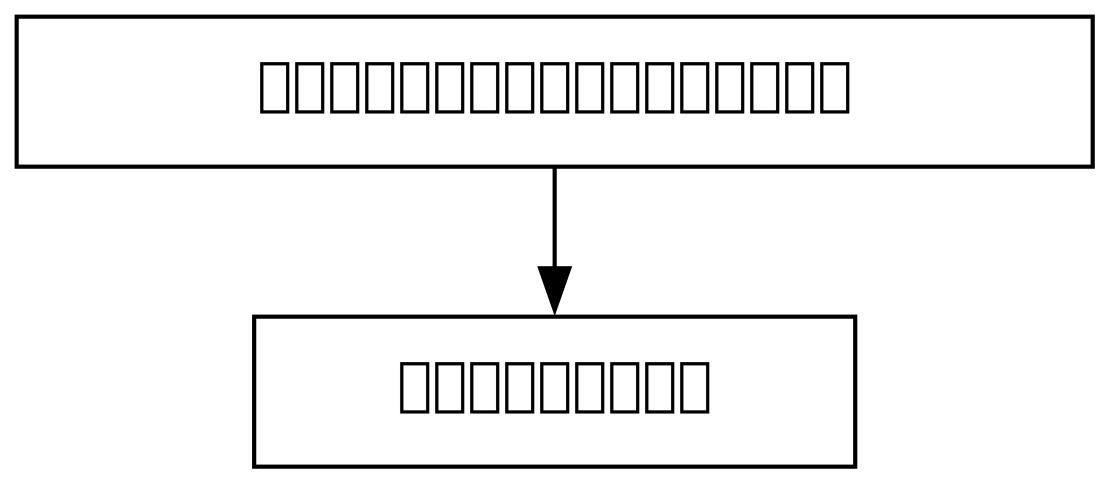
\includegraphics[keepaspectratio, width=0.8\linewidth]{figures/sato/AdminGetNotReportNumber.pdf}
    \caption{AdminGetNotReportNumber}
    \label{fig:AdminGetNotReportNumber}
\end{figure}
\subsubsection{ProcessReportDeletePinDetail}
\begin{figure}[H]
    \centering
    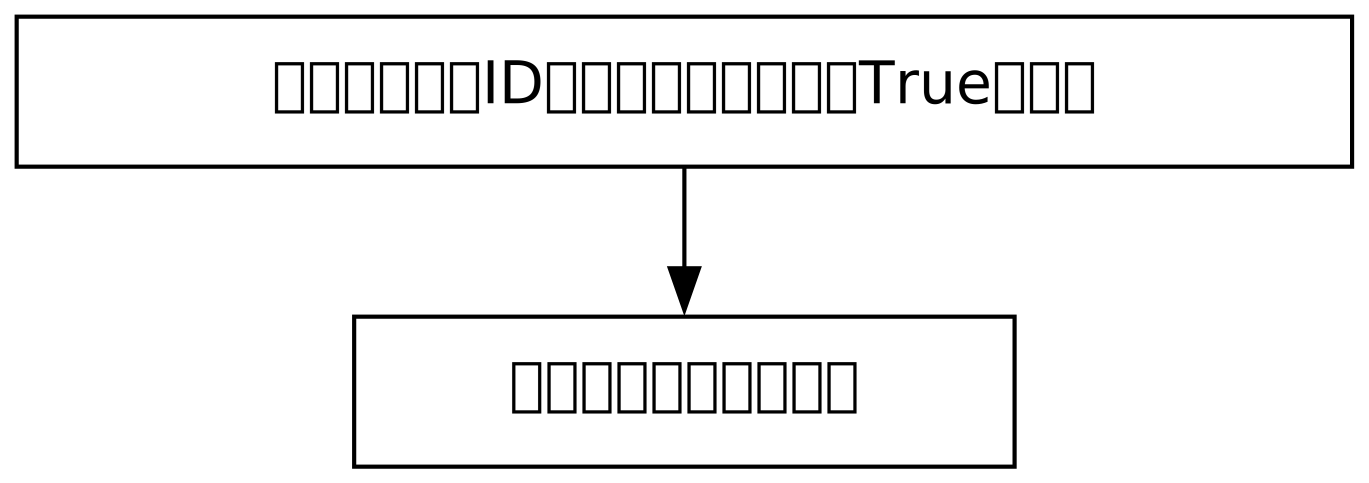
\includegraphics[keepaspectratio, width=0.8\linewidth]{figures/sato/ProcessReportDeletePinDetail.pdf}
    \caption{ProcessReportDeletePinDetail}
    \label{fig:ProcessReportDeletePinDetail}
\end{figure}
\subsubsection{InputBusinessInformation}
\begin{figure}[H]
    \centering
    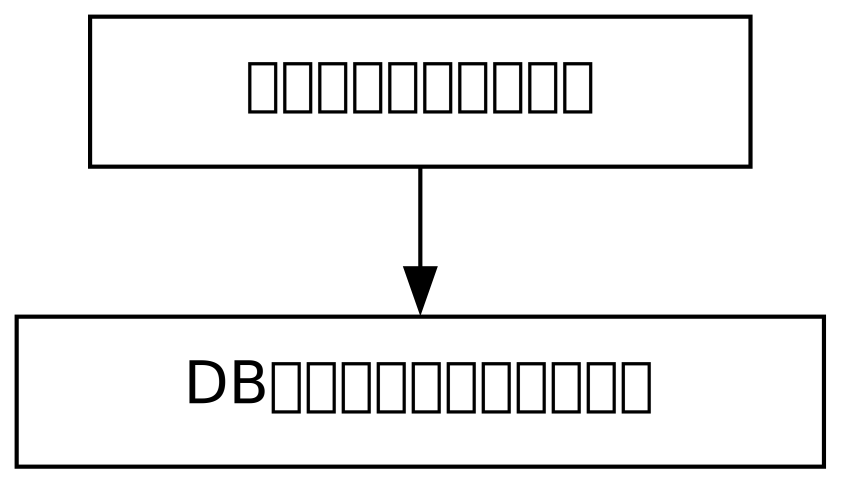
\includegraphics[keepaspectratio, width=0.8\linewidth]{figures/sato/InputBusinessInformation.pdf}
    \caption{InputBusinessInformation}
    \label{fig:InputBusinessInformation}
\end{figure}
\subsubsection{AdminDeleletePost}
\begin{figure}[H]
    \centering
    \includegraphics[keepaspectratio, width=0.8\linewidth]{figures/sato/AdminDeleletePost.pdf}
    \caption{AdminDeleletePost}
    \label{fig:AdminDeleletePost}
\end{figure}
\subsubsection{SendUserMessage}
\begin{figure}[H]
    \centering
    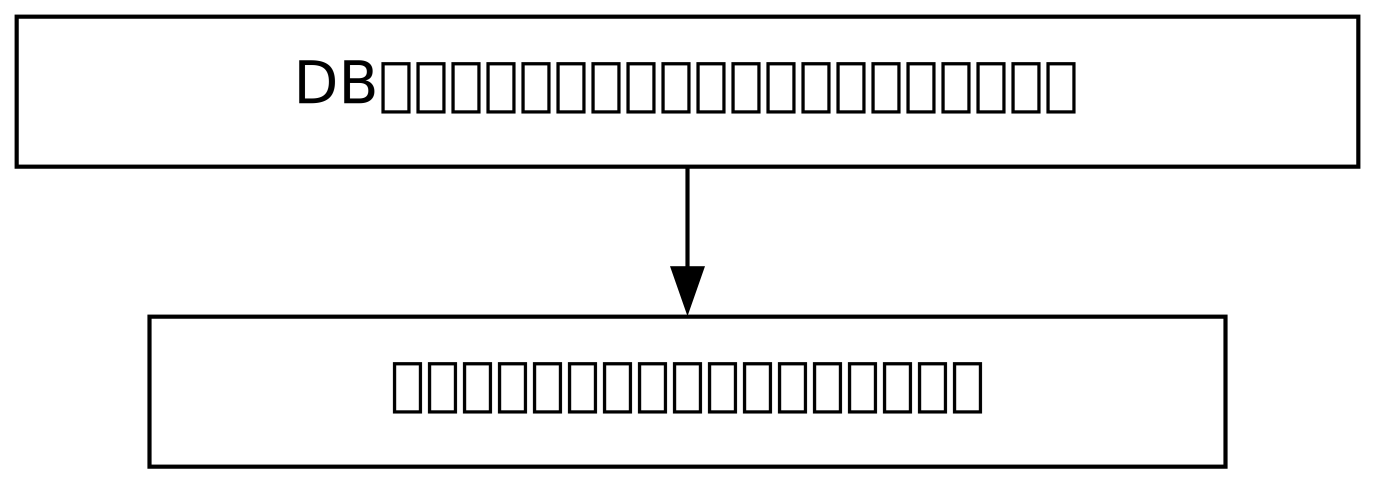
\includegraphics[keepaspectratio, width=0.8\linewidth]{figures/sato/SendUserMessage.pdf}
    \caption{SendUserMessage}
    \label{fig:SendUserMessage}
\end{figure}
\subsubsection{AdminDeleteAccount}
\begin{figure}[H]
    \centering
    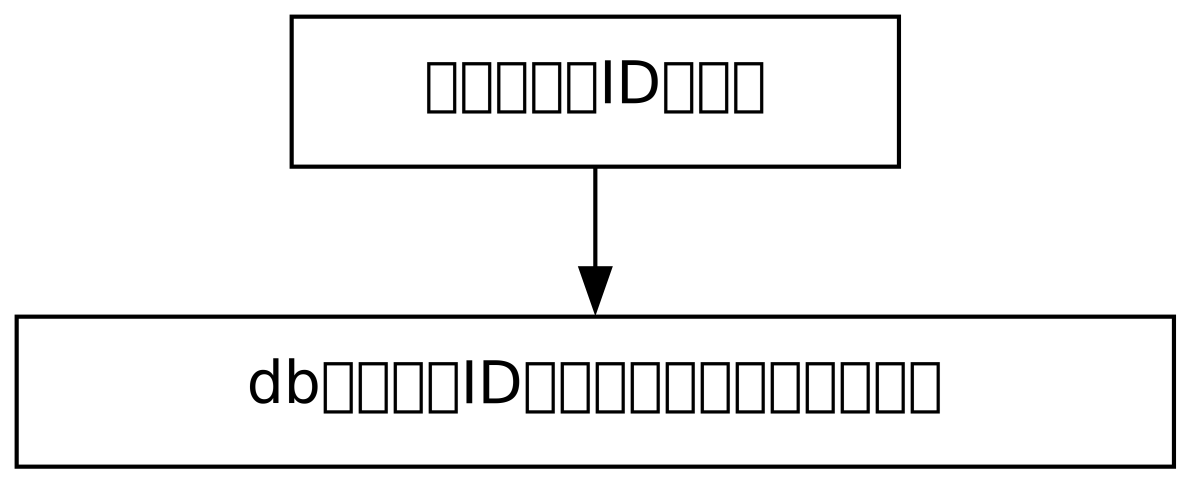
\includegraphics[keepaspectratio, width=0.8\linewidth]{figures/sato/AdminDeleteAccount.pdf}
    \caption{AdminDeleteAccount}
    \label{fig:AdminDeleteAccount}
\end{figure}
\subsubsection{ProcessContact}
\begin{figure}[H]
    \centering
    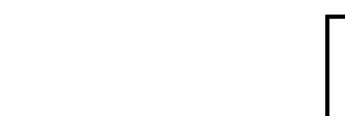
\includegraphics[keepaspectratio, width=0.8\linewidth]{figures/sato/ProcessContact.pdf}
    \caption{ProcessContact}
    \label{fig:ProcessContact}
\end{figure}
\subsubsection{SendUserMailContact}
\begin{figure}[H]
    \centering
    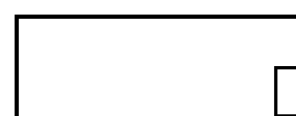
\includegraphics[keepaspectratio, width=0.8\linewidth]{figures/sato/SendUserMailContact.pdf}
    \caption{SendUserMailContact}
    \label{fig:SendUserMailContact}
\end{figure}

% データベース設計

\end{document}